\chapter{Business process management}

\begin{description}
    \item[Information system] \marginnote{Information system}
        Contains static (raw) data partially describing the flow of a business.

    \item[Business process management] \marginnote{Business process management}
        Methods to design, manage and analyze business processes by mining data contained in information systems.

        Business processes help in making decisions and automations.

    \item[Business process lifecycle] \phantom{}
        \begin{description}
            \item[Design and analysis]
                Definition of models and schemas.
            \item[Configuration]
                Execution of the business process.
            \item[Enactment]
                Collect and analyze logs to make predictions.
            \item[Evaluation]
                Assess the quality of the process.
        \end{description}

    \item[Business process types] \phantom{}
        \begin{description}
            \item[Organizational vs operational] \phantom{} 
                \begin{description}
                    \item[Organizational]
                        Process described with its inputs, outputs, expected outcomes and dependencies.
                    \item[Operational]
                        Process described disregarding its implementation.
                \end{description}

            \item[Intra-organization vs inter-organization] \phantom{}
                \begin{description}
                    \item[Intra-organization]
                        Only activities executed within the business boundaries.
                    \item[Inter-organization]
                        Part of the activities are executed outside the business and the process does not have control of them.
                \end{description}

            \item[Execution properties] \phantom{}
                \begin{description}
                    \item[Degree of automation] 
                    \item[Degree of repetition] 
                    \item[Degree of structuring] 
                \end{description}
        \end{description}
\end{description}



\section{Business process modelling}

\begin{description}
    \item[Activity instance] \marginnote{Activity instance}
        Represents the actual work done during the execution of a business process.

        An activity instance can be described as a sequence of temporally ordered events.
        Formally, an activity instance $i$ is defined as:
        \[ i = (E_i, <_i) \]
        where $E_i \subseteq \{ i_i, e_i, b_i, t_i \}$ is an event with:
        \begin{itemize}
            \item $i_i$ for initialization;
            \item $e_i$ for enabling;
            \item $b_i$ for beginning;
            \item $t_i$ for terminating.
        \end{itemize}
        $<_i$ is a relation order such that $<_i \subseteq \{ (i_i, e_i), (e_i, b_i), (b_i, t_i) \}$.

    \item[Activity model] \marginnote{Activity model}
        Describes a set of similar activity instances.
\end{description}


\subsection{Control flow modelling}

\begin{description}
    \item[Process modelling types] \phantom{}
        \begin{description}
            \item[Procedural vs declarative] \phantom{}
                \begin{description}
                    \item[Procedural] \marginnote{Procedural modelling}
                        Based on a strict ordering of the steps.
                        Uses conditional choices, loops, parallel execution, events. 

                        Subject to the spaghetti-like process problem.

                    \item[Declarative] \marginnote{Declarative modelling}
                        Based on the properties that should hold during execution.
                        Uses concepts as: executions, expected executions, prohibited executions.
                \end{description}

            \item[Closed vs open] \phantom{}
                \begin{description}
                    \item[Closed] \marginnote{Closed modelling}
                        The execution of non-modelled activities is prohibited.
                    
                    \item[Open] \marginnote{Open modelling}
                        Constraints to allow non-modelled activities.
                \end{description}
        \end{description}
\end{description}

The most common combination of approaches are:
\begin{descriptionlist}
    \item[Closed procedural process modelling] 
    \item[Open declarative process modelling] 
\end{descriptionlist}



\section{Closed procedural process modelling}

\begin{description}
    \item[Process model]
        Set of process instances with a similar structure described as a graph.

        \begin{description}
            \item[Edges] Directed arcs to describe temporal orderings.
            
            \item[Nodes] Nodes can be:
                \begin{description}
                    \item[Activity models] \marginnote{Activity} 
                        Unit of work.
                    \item[Event models] \marginnote{Event} 
                        Capture the events that involve activities.
                    \item[Gateway models] \marginnote{Gateway} 
                        Control flow constructs.
                        Basic patterns are: \texttt{sequence}, \texttt{and split}, \texttt{and join}, \texttt{exclusive or split}, \texttt{exclusive or join}
                \end{description}
        \end{description}

        \begin{example}
            Activity $A$ is executed before activity $B$ (\texttt{sequence} arc).
            \begin{center}
                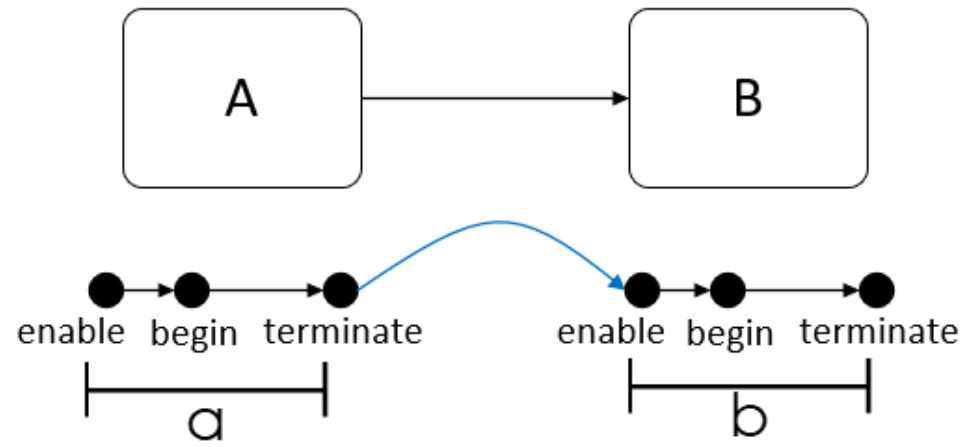
\includegraphics[width=0.4\textwidth]{img/bp_control_flow_sequence.png}
            \end{center}
        \end{example}

        \begin{example}
            Loop with \texttt{exclusive or splits}.
            \begin{center}
                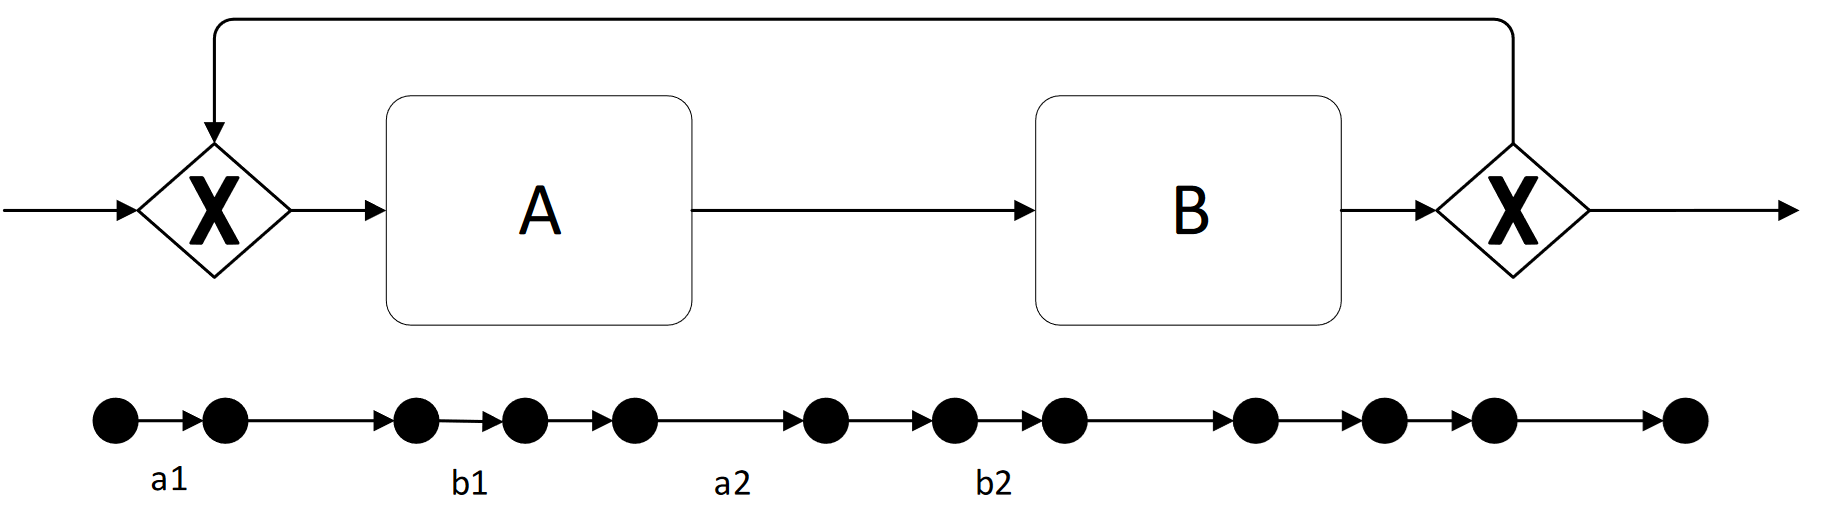
\includegraphics[width=0.5\textwidth]{img/bp_control_flow_loop.png}
            \end{center}
        \end{example}

        \begin{example} \phantom{}\\
            \begin{minipage}{0.49\textwidth}
                The \texttt{and split} allows to run $B$ and $C$ in parallel.
                \begin{center}
                    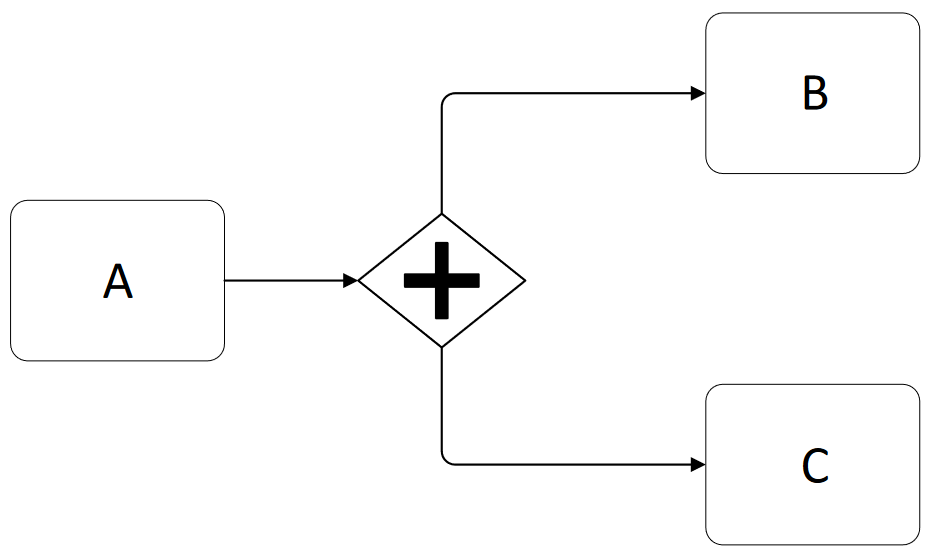
\includegraphics[width=0.6\linewidth]{img/bp_control_flow_parallel_split.png}
                \end{center}
            \end{minipage}
            \hspace{0.02\textwidth}
            \begin{minipage}{0.49\textwidth}
                The \texttt{and join} allows to wait for both $B$ and $C$ to finish.
                \begin{center}
                    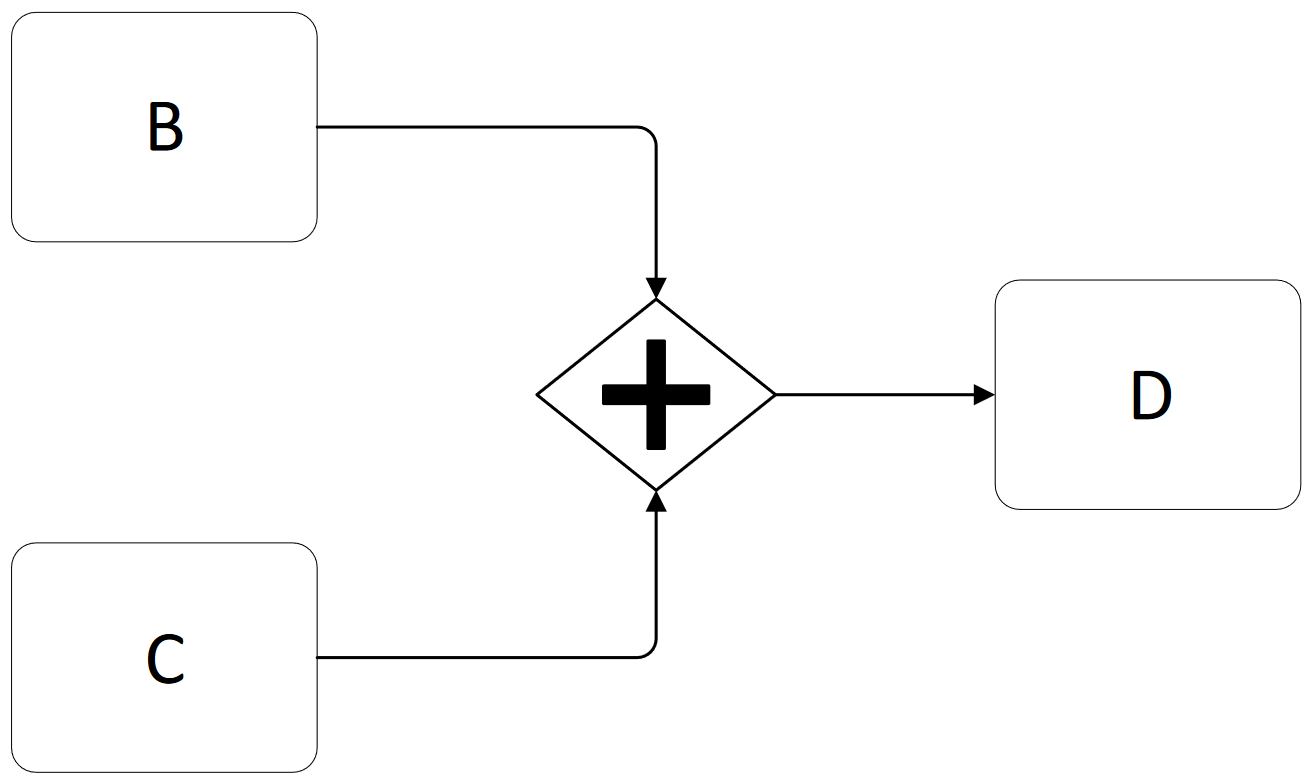
\includegraphics[width=0.6\linewidth]{img/bp_control_flow_parallel_join.png}
                \end{center}
            \end{minipage}
        \end{example}

        \begin{example} \phantom{}\\
            \begin{minipage}{0.49\textwidth}
                The \texttt{xor split} allows to run only one activity between $B$ and $C$.
                \begin{center}
                    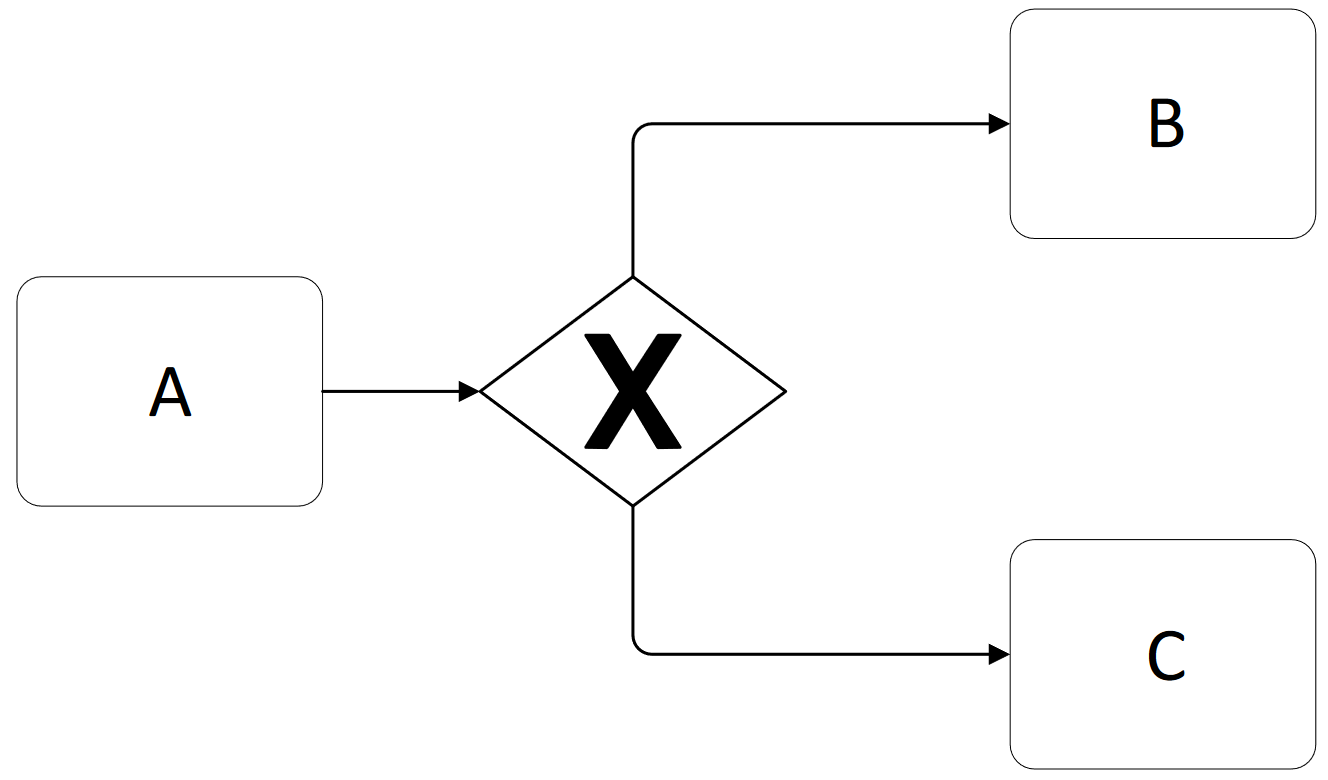
\includegraphics[width=0.6\linewidth]{img/bp_control_flow_xor_split.png}
                \end{center}
            \end{minipage}
            \hspace{0.02\textwidth}
            \begin{minipage}{0.49\textwidth}
                The \texttt{xor join} allows to wait for one activity between $B$ and $C$ to finish.
                \begin{center}
                    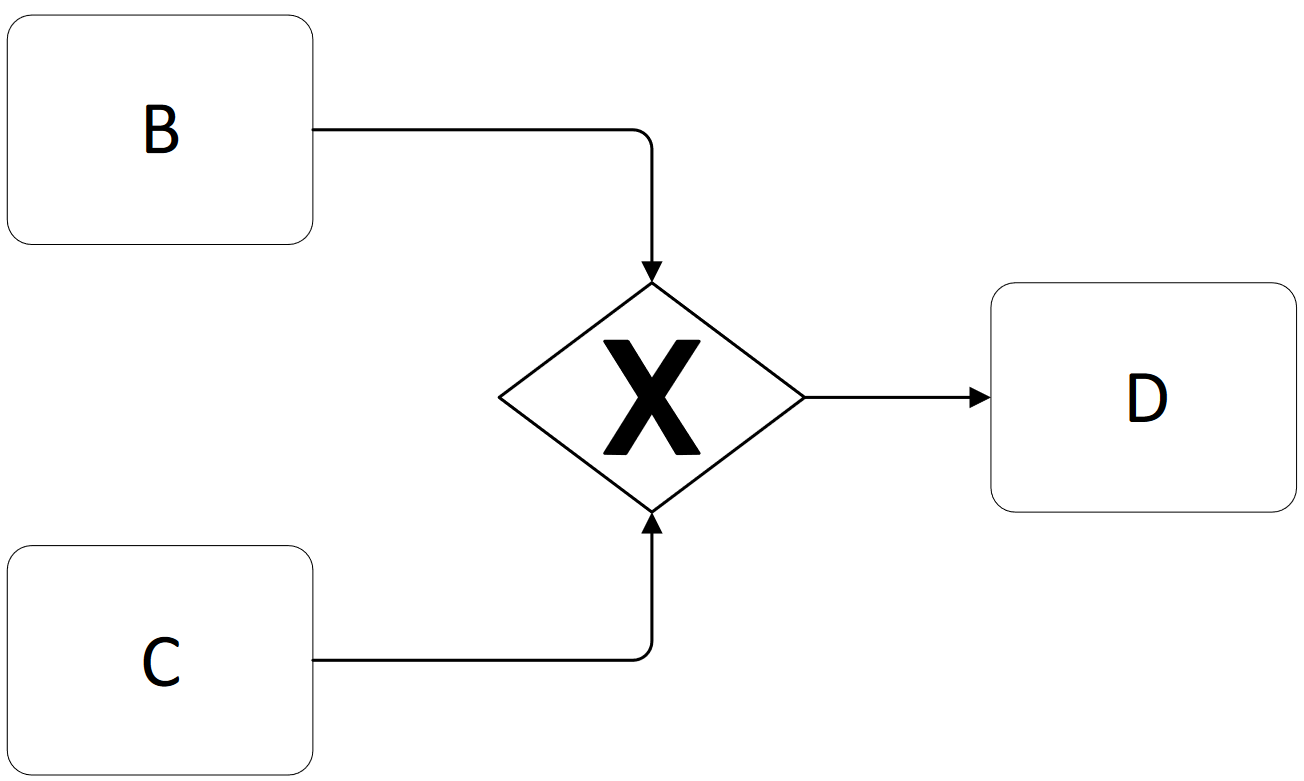
\includegraphics[width=0.6\linewidth]{img/bp_control_flow_xor_join.png}
                \end{center}
            \end{minipage}
        \end{example}

        \begin{example}
            The \texttt{or split} allows to run at least one activity between $B$ and $C$.
            \begin{center}
                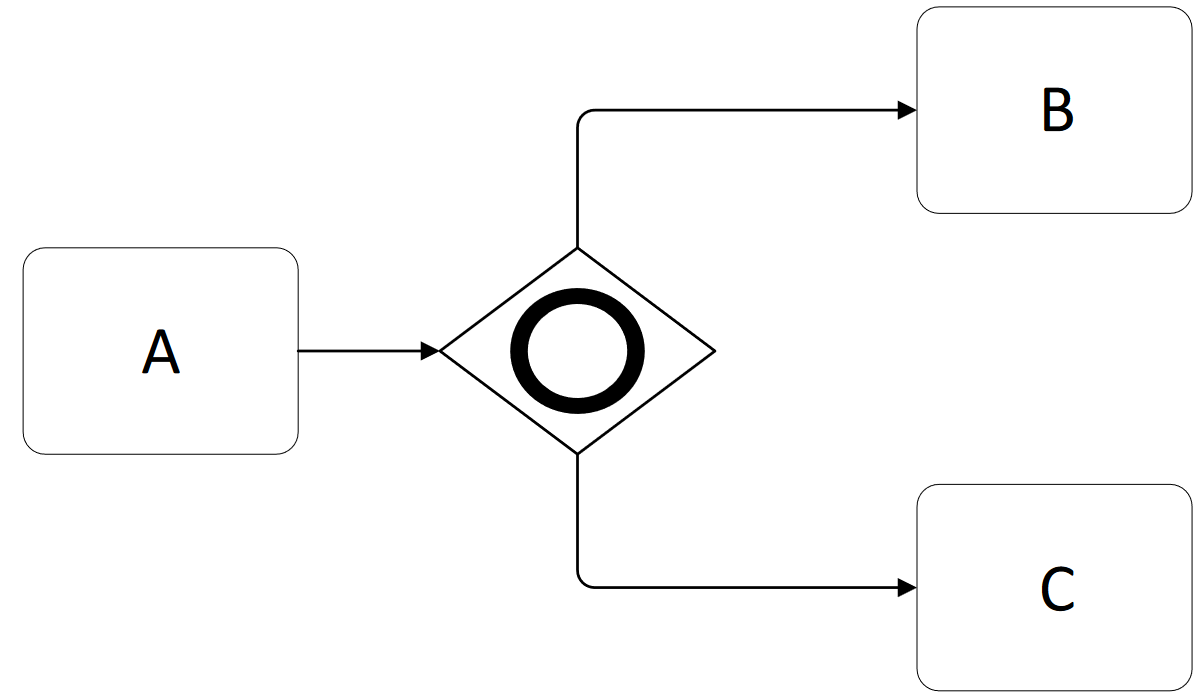
\includegraphics[width=0.3\textwidth]{img/bp_control_flow_or_split.png}
            \end{center}
        \end{example}

        \begin{example}
            The \texttt{N-out-of-M join} allows to wait until $N$ activities have finished.
            \begin{center}
                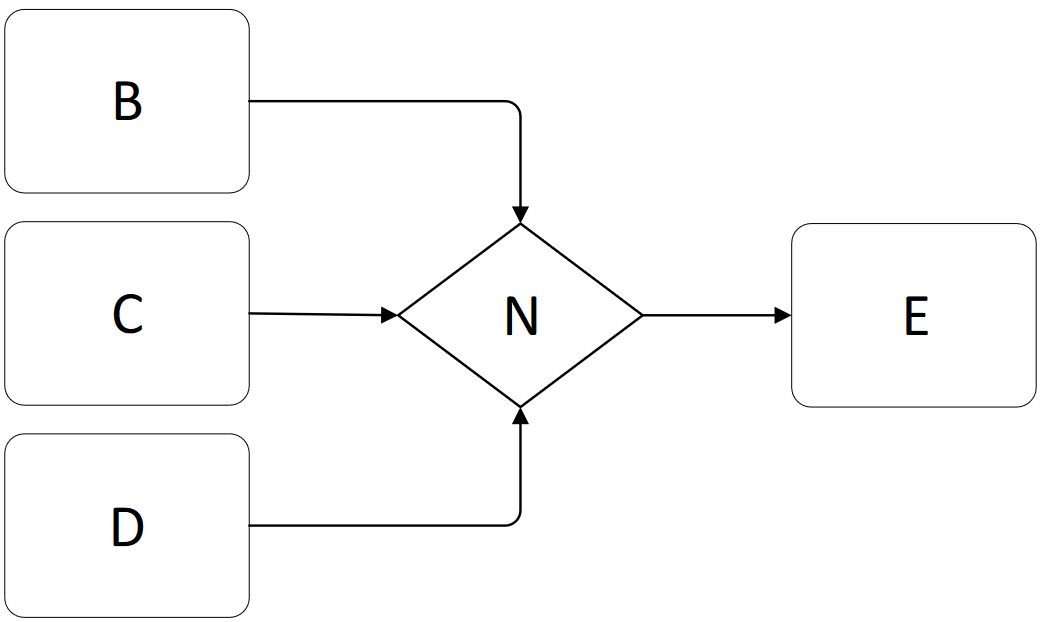
\includegraphics[width=0.3\textwidth]{img/bp_control_flow_n_out_of_m_join.png}
            \end{center}
        \end{example}
\end{description}



\subsection{Petri nets}

\begin{description}
    \item[Places] \marginnote{Places}
        Represent the points of execution of a process.
        Drawn as empty circles.

    \item[Tokens] \marginnote{Tokens}
        A token can reside in a place.
        It marks the current state of the process.
        Drawn as a small black circle.
    
    \item[Transitions] \marginnote{Transitions}
        Have input and output places.
        Drawn as rectangles.

        \begin{description}
            \item[Token play]
                A transition is enabled when all the input places of a transition have a token and all the output places have not.
                An enabled transition can be fired: tokens are removed from the inputs and moved to the outputs.
        \end{description}

    \item[Connections] \marginnote{Connections}
        Arcs to connect places and transitions.
\end{description}

\begin{example} \phantom{}
    \begin{center}
        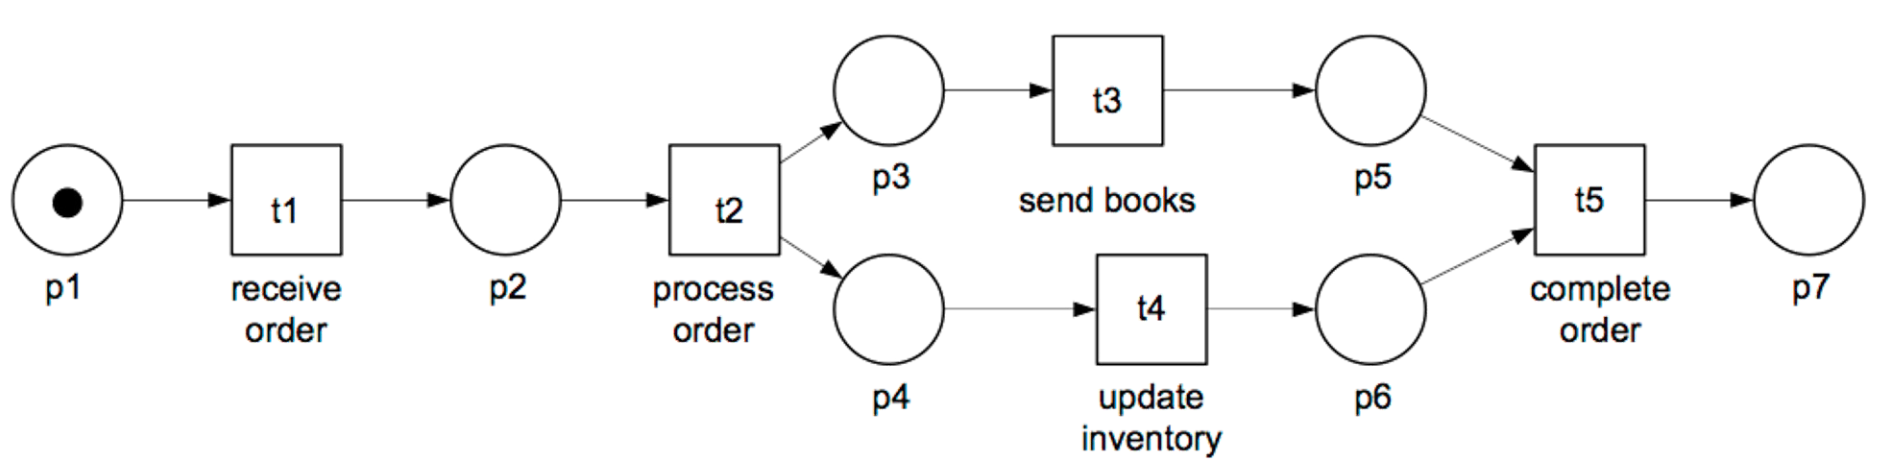
\includegraphics[width=0.65\textwidth]{img/petri_net_example1.png}
    \end{center}
    Transition $t_2$ is a split. $t_5$ is a join.
\end{example}

\begin{table}[H]
    \centering
    \begin{tabular}{c|c}
        \textbf{Petri nets} & \textbf{Business process modelling} \\
        \hline
        Petri net & Process model \\
        Transitions & Activity models \\
        Tokens & Instances \\
        Transition firing & Activity execution \\
    \end{tabular}
    \caption{Petri nets and business process modelling concepts equivalence}
\end{table}


\subsection{Workflow nets}
Restriction of Petri nets.

\begin{description}
    \item[Transitions syntactic sugar] \marginnote{Transitions} \phantom{}
        \begin{center}
            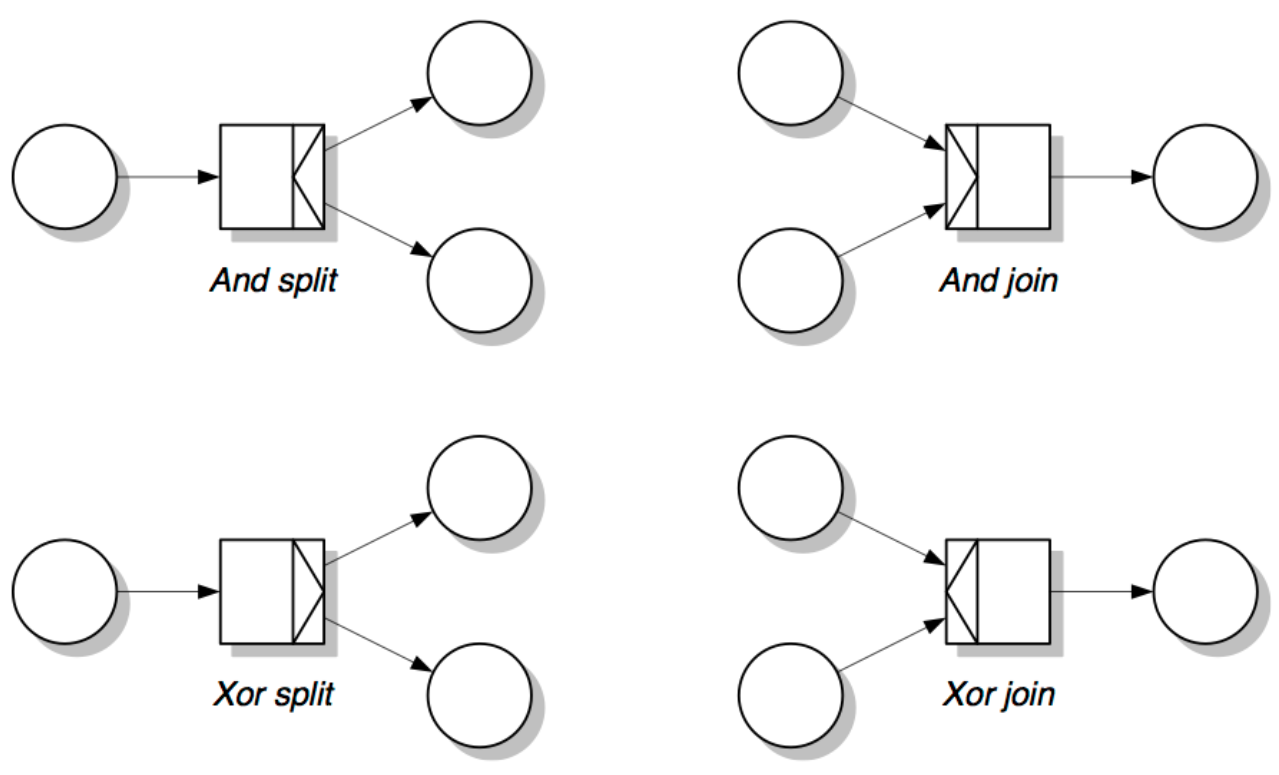
\includegraphics[width=0.5\textwidth]{img/workflow_nets_transitions.png}
        \end{center}

    \item[Triggers] \marginnote{Triggers} 
        Can be attached to transitions.
        \begin{description}
            \item[Automatic trigger] Activity started automatically (standard behavior).

            \item[User trigger] Activity started on user input.
                \begin{center}
                    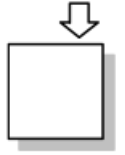
\includegraphics[width=0.6cm]{img/workflow_nets_user_trigger.png}
                \end{center}

            \item[External trigger] Activity started on external events.
                \begin{center}
                    
\includegraphics[width=0.6cm]{img/workflow_nets_external_trigger.png}
                \end{center}

            \item[Time trigger] Activity started at a certain time.
                \begin{center}
                    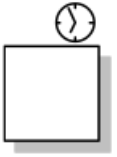
\includegraphics[width=0.6cm]{img/workflow_nets_time_trigger.png}
                \end{center}
        \end{description}
\end{description}


\begin{example}[Workflow nets with explicit and implicit \texttt{exclusive or split}]
    \begin{center}
        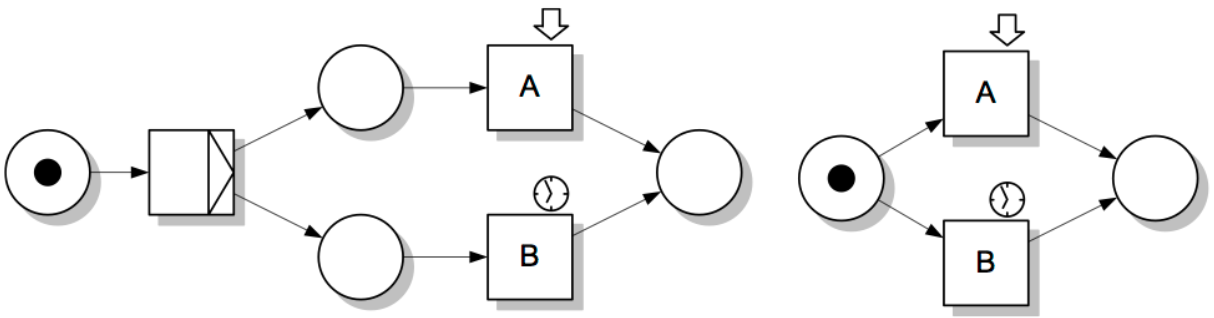
\includegraphics[width=0.6\textwidth]{img/workflow_nets_example1.png}
    \end{center}
\end{example}



\subsection{Business process model and notation (BPMN)}
De-facto standard for business process representation.

\begin{description}
    \item[Basic elements] \phantom{}
        \begin{description}
            \item[Activity] \marginnote{Activity}
                Drawn as rectangles with optional decorations (e.g. a decorator to represent a task under human responsibility).
            
            \item[Event] \marginnote{Event}
                Drawn as circles.

                \begin{description}
                    \item[Start event]
                        Indicates where and how (triggers) a process starts.
                        Drawn as a thin-bordered circle.
                    
                    \item[Intermediate event]
                        Event occurring after the start of a process, but before its end.

                    \item[End event]
                        Indicates the end of a process and optionally provides its result.
                        Drawn as a thick-bordered circle.
                \end{description}
            
            \item[Flow] \marginnote{Flow}
                Drawn as arrows.

                \begin{description}
                    \item[Sequence flow] 
                        Flow of processes (orchestration).

                    \item[Message flow] 
                        Communication between processes and external entities.
                \end{description}
            
            \item[Gateway] \marginnote{Gateway}
                Parallel, split and join. Drawn as rhombus.
        \end{description}

    \item[Pool] \marginnote{Pool}
        Represent an independent participant with its own business process specification.
    
    \item[Lanes] \marginnote{Lanes}
        Resource classes within a pool.
    
    \item[Data] \marginnote{Data} \phantom{}
        \begin{description}
            \item[Data object] Local variable representing a temporary unit of information.
            \item[Data object reference] Reference to a data object.
            \item[Data object collection] Collection of data objects.
            \item[Data store] Persistent unit of information accessed by the process and external entities.
        \end{description}
        \begin{figure}[H]
            \centering
            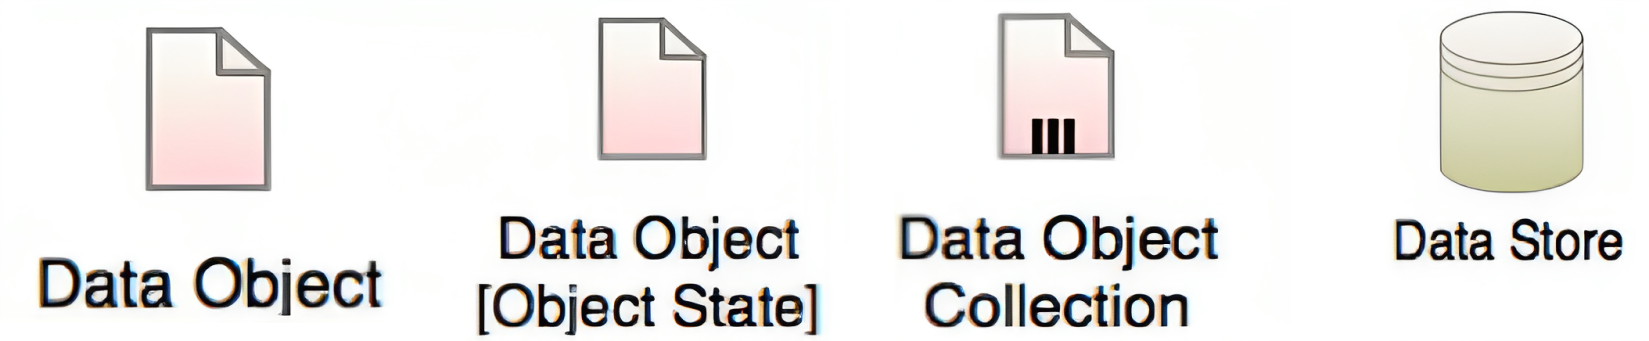
\includegraphics[width=0.4\textwidth]{img/bpmn_data.png}
            \caption{Data symbols}
        \end{figure}

    \item[Reaction to events] \marginnote{Reactions} \phantom{}
        \begin{description}
            \item[Throw] Signals that something happened. 
            \item[Catch] Responds to a signal.
        \end{description}
\end{description}

\begin{figure}[H]
    \centering
    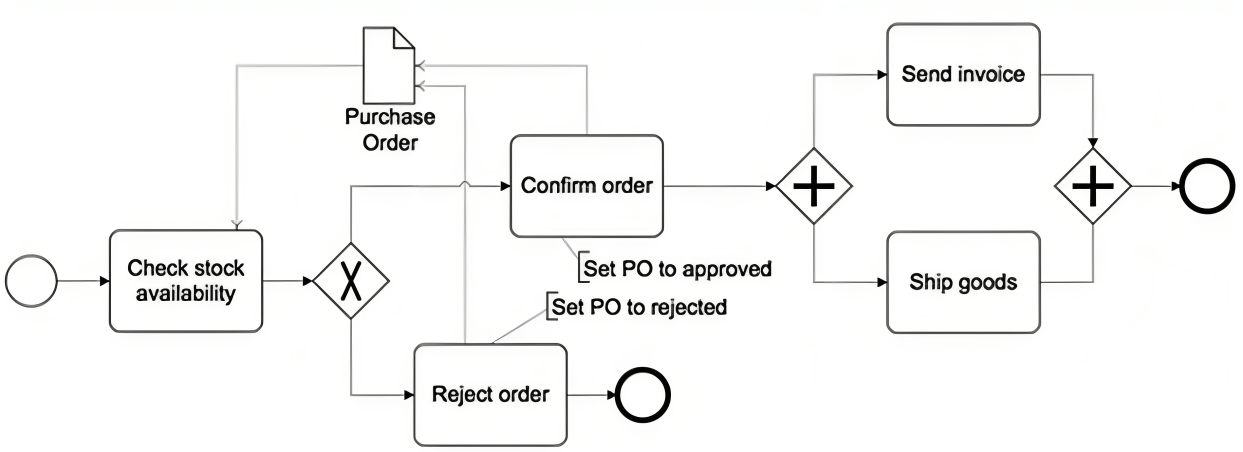
\includegraphics[width=0.6\textwidth]{img/bpmn_example1.png}
    \caption{Example of BPMN}
\end{figure}



\section{Open declarative process modelling}

Define formal properties for process models (i.e. more formal than procedural methods).
Properties defined in term of the evolution of the process (similar to the evolution of the world in modal logics)


\subsection{Linear-time temporal logic in BPM}
Based on the notion of world. Advancements in the process result in new worlds.

\begin{description}
    \item[LTL model] \marginnote{LTL model}
        An LTL model is a set of events that happened in the execution of an instance of a process.

    \item[LTL execution trace] \marginnote{LTL execution trace}
        An LTL execution trace is an LTL model based on the set of natural numbers.
        It represents the evolution of the world.

    \item[Syntax and semantics] Follows from the syntax and semantics of linear-time temporal logic.
\end{description}


\subsection{DECLARE}

Based on constraints that must hold in every possible execution of the system.

\begin{description}
    \item[Atomic activity] \marginnote{Atomic activity}
        Drawn as boxes.
    
    \item[Unary constraints] \marginnote{Unary constraints}
        Defined on atomic activities.
        \begin{center}
            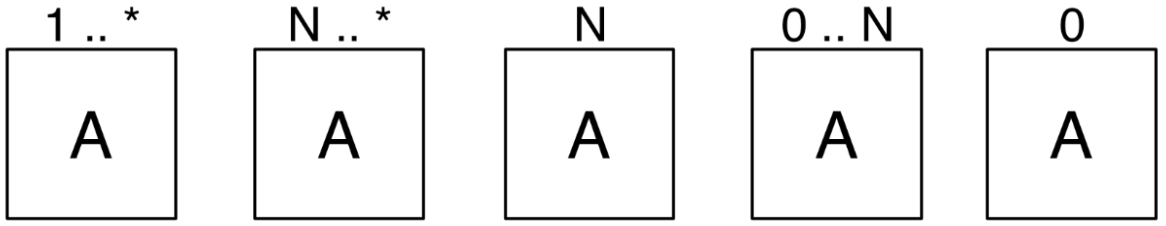
\includegraphics[width=0.4\textwidth]{img/declare_unary_constraint.png}
        \end{center}

    \item[Binary constraints] \marginnote{Binary constraints}
        Connects two activities.

        A solid circle indicates when the constraint is enforced.
        A directed arrow indicates time ordering.

        \begin{description}
            \item[Response] 
                An execution of $A$ should be eventually followed by an execution of $B$.
                \begin{center}
                    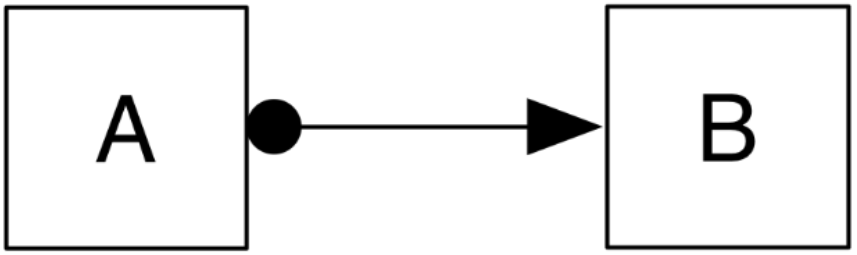
\includegraphics[width=0.2\textwidth]{img/declare_response.png}
                \end{center}

            \item[Chained response] 
                An execution of $A$ should be immediately followed by an execution of $B$.
                \begin{center}
                    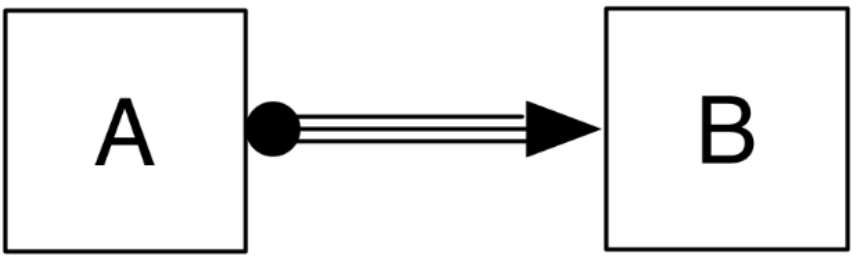
\includegraphics[width=0.2\textwidth]{img/declare_chained_response.png}
                \end{center}

            \item[Negated response] 
                After the execution of $A$, $B$ cannot be executed anymore.
                \begin{center}
                    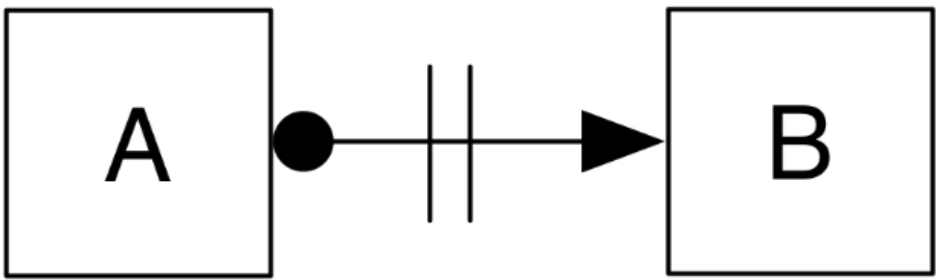
\includegraphics[width=0.2\textwidth]{img/declare_negated_response.png}
                \end{center}

            \item[Precedence] 
                An execution of $B$ should have been preceded by an execution of $A$.
                \begin{center}
                    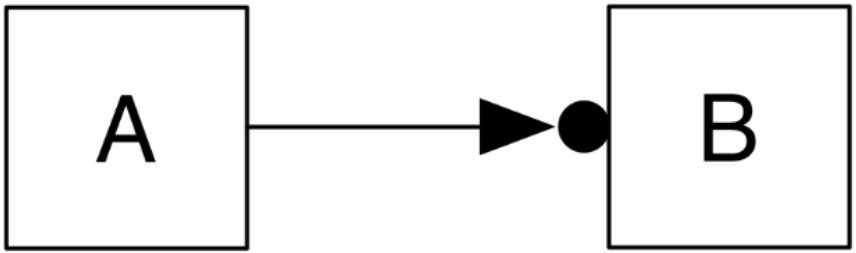
\includegraphics[width=0.2\textwidth]{img/declare_precedence.png}
                \end{center}
        \end{description}

    \item[Semantics]
        The semantic of the constraints can be defined using LTL.

    \item[Verifiable properties] \phantom{}
        \begin{description}
            \item[Enactment] \marginnote{Enactment} 
                Determine the next possible activities.
            \item[Conformance] \marginnote{Conformance} 
                Check if an instance of a process respects the constraints.
            \item[Interoperability] \marginnote{Interoperability} 
                Determine if two DECLARE systems can be merged.
        \end{description}

    \item[Limits] \phantom{}
        \begin{itemize}
            \item DECLARE cannot represent quantitative temporal constraints.
            \item Compared to closed procedural methods, it is more difficult to learn models.
        \end{itemize}
\end{description}



\section{Business process mining}

\begin{description}
    \item[Event log] \marginnote{Event log}
        Sequence of events.
        Each event (trace) is a sequence of activities.

        \begin{example}
            $L = \{ \langle \texttt{abcd} \rangle, \langle \texttt{abcd} \rangle, \langle \texttt{acbd} \rangle \}$
        \end{example}

    \item[Business process mining] \marginnote{Business process mining}
        Extract knowledge from event logs to improve a process.

        Possible applications are:
        \begin{itemize}
            \item Automated process discovery.
            \item Conformance checking.
            \item Organizational mining.
            \item Simulations.
            \item Process extension.
            \item Predictions.
        \end{itemize}

    \item[Process mining types] \phantom{}
        \begin{description}
            \item[Discovery] \marginnote{Discovery}
                Takes as input an event log and outputs a model.
                \begin{center}
                    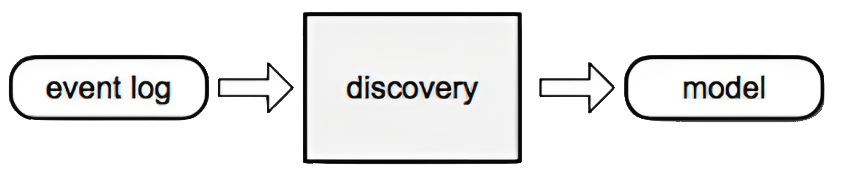
\includegraphics[width=0.4\textwidth]{img/process_mining_discovery.png}
                \end{center}

            \item[Conformance checking] \marginnote{Conformance checking}
                Takes as input an event log and a model and outputs if the log is conformant to the model.
                \begin{center}
                    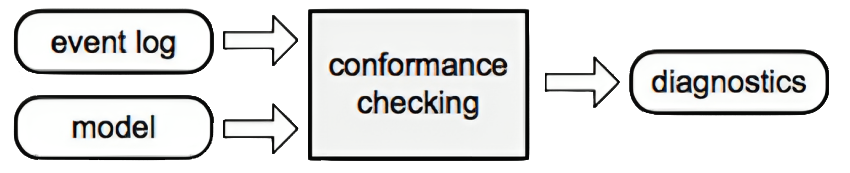
\includegraphics[width=0.4\textwidth]{img/process_mining_conformance.png}
                \end{center}

            \item[Enhancement] \marginnote{Enhancement}
                Takes as input an event log and a model and outputs a new model.
                \begin{center}
                    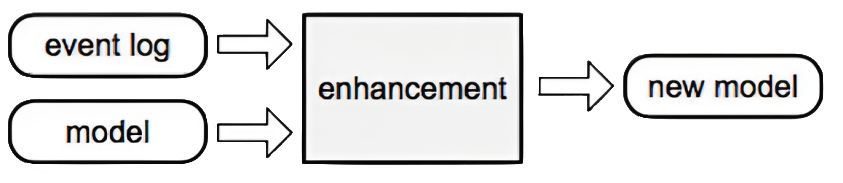
\includegraphics[width=0.4\textwidth]{img/process_mining_enhancement.png}
                \end{center}
        \end{description}
\end{description}


\subsection{Process discovery}

\begin{description}
    \item[Process discovery] \marginnote{Process discovery}
        Learn a process model representative of the input event log.

        More formally, a process discovery algorithm is a function that maps an event log into a business process modelling language.
        In our case, we map logs into Petri nets (preferably workflow nets).

        \begin{remark}
            Process discovery is a unary classification problem.
            We are interested in learning a model fitted on the entire event log.
        \end{remark}

    \item[$\alpha$-algorithm] \marginnote{$\alpha$-algorithm}
        $\alpha$-algorithm fixes the following interesting relations:
        \begin{descriptionlist}
            \item[$>_L$)] $a >_L b$ iff there exists a trace in the event log where $a$ precedes $b$.
            \item[$\rightarrow_L$)] $a \rightarrow_L b$ iff $a >_L b$ and $b \cancel{>}_L\, a$.
            \item[$\#_L$)] $a \# b$ iff $a \cancel{>}_L\, b$ and $b \cancel{>}_L\, a$.
            \item[$\Vert_L$)] $a \Vert_L b$ iff $a >_L b$ and $b >_L a$.
        \end{descriptionlist}

        $\alpha$-algorithm works as follows:
        \begin{enumerate}
            \item Look for the relations in the event log.
            \item Focus on the most interesting relations and identify the biggest set of involved activities.
            \item Remove redundancies.
            \item Represent them as a Petri net.
        \end{enumerate}

        \begin{example}
            Given the event log $L = \{ \langle \texttt{abcd} \rangle, \langle \texttt{abcd} \rangle, 
            \langle \texttt{abcd} \rangle, \langle \texttt{acbd} \rangle, \langle \texttt{acbd} \rangle, \langle \texttt{aed} \rangle \}$,
            we want to apply the $\alpha$-algorithm:
            \begin{enumerate}
                \item We determine the relations:
                    \[ 
                        \begin{split}
                            >_{L_1} &= \{ (\texttt{a}, \texttt{b}), (\texttt{a}, \texttt{c}), (\texttt{a}, \texttt{e}), (\texttt{b}, \texttt{c}),
                                    (\texttt{c}, \texttt{b}), (\texttt{b}, \texttt{d}), (\texttt{c}, \texttt{d}), (\texttt{e}, \texttt{d}) \} \\
                            \rightarrow_{L_1} &= \{ (\texttt{a}, \texttt{b}), (\texttt{a}, \texttt{c}), (\texttt{a}, \texttt{e}), 
                                                (\texttt{b}, \texttt{d}), (\texttt{c}, \texttt{d}), (\texttt{e}, \texttt{d}) \} \\
                            \#_{L_1} &= \{ (\texttt{a}, \texttt{a}), (\texttt{a}, \texttt{d}), (\texttt{b}, \texttt{b}), (\texttt{b}, \texttt{e}), (\texttt{c}, \texttt{c}), 
                                (\texttt{c}, \texttt{e}), (\texttt{d}, \texttt{a}), (\texttt{d}, \texttt{d}), (\texttt{e}, \texttt{b}), (\texttt{e}, \texttt{c}), (\texttt{e}, \texttt{e}) \} \\
                            \Vert_{L_1} &= \{ (\texttt{b}, \texttt{c}), (\texttt{c}, \texttt{b}) \} 
                        \end{split} 
                    \]
                    And construct the footprint matrix:
                    \begin{center}
                        \begin{tabular}{c | c c c c c}
                                        & \texttt{a}            & \texttt{b}            & \texttt{c}            & \texttt{d}            & \texttt{e} \\
                            \hline
                            \texttt{a}  & $\#_{L_1}$            & $\rightarrow_{L_1}$   & $\rightarrow_{L_1}$   & $\#_{L_1}$            & $\rightarrow_{L_1}$ \\
                            \texttt{b}  & $\leftarrow_{L_1}$    & $\#_{L_1}$            & $\Vert_{L_1}$         & $\rightarrow_{L_1}$   & $\#_{L_1}$ \\
                            \texttt{c}  & $\leftarrow_{L_1}$    & $\Vert_{L_1}$         & $\#_{L_1}$            & $\rightarrow_{L_1}$   & $\#_{L_1}$ \\
                            \texttt{d}  & $\#_{L_1}$            & $\leftarrow_{L_1}$    & $\leftarrow_{L_1}$    & $\#_{L_1}$            & $\leftarrow_{L_1}$ \\
                            \texttt{e}  & $\leftarrow_{L_1}$    & $\#_{L_1}$            & $\#_{L_1}$            & $\rightarrow_{L_1}$   & $\#_{L_1}$ \\
                        \end{tabular}
                    \end{center}

                \item We determine the interesting relations as the pair of sets $(P, Q)$ of activities such that:
                    \[ \forall p \in P, q \in Q: (p \rightarrow q) \land (p \# p) \land (q \# q) \]
                    
                    This can be algorithmically done by building a footprint table whose rows and columns allow to obtain all the combinations of the activities.
                    Therefore, the set of interesting relations is:
                    \[
                        \begin{split}
                            X_{L_1} = \{ 
                                (\{\texttt{a}\}, \{\texttt{b}\}), (\{\texttt{a}\}, \{\texttt{c}\}), (\{\texttt{a}\}, \{\texttt{e}\}), 
                                (\{\texttt{a}\}, \{\texttt{b}, \texttt{e}\}), (\{\texttt{a}\}, \{\texttt{c}, \texttt{e}\}), \\
                                (\{\texttt{b}\}, \{\texttt{d}\}), (\{\texttt{c}\}, \{\texttt{d}\}), (\{\texttt{e}\}, \{\texttt{d}\}), 
                                (\{\texttt{b}, \texttt{e}\}, \{\texttt{d}\}), (\{\texttt{c}, \texttt{e}\}, \{\texttt{d}\}) 
                            \} 
                        \end{split}
                    \]

                \item Then, we remove the redundancies in the set of interesting relations $X_{L_1}$:
                    \[ Y_{L_1} = \{ (\{\texttt{a}\}, \{\texttt{b}, \texttt{e}\}), (\{\texttt{a}\}, \{\texttt{c}, \texttt{e}\}),
                        (\{\texttt{b}, \texttt{e}\}, \{\texttt{d}\}), (\{\texttt{c}, \texttt{e}\}, \{\texttt{d}\}) \} \]
                    It can be seen that all the relations in $X_{L_1}$ can be derived from $Y_{L_1} \subset X_{L_1}$.
                
                \item With the reduced set of interesting relations, we can build the Petri net.
                    \begin{center}
                        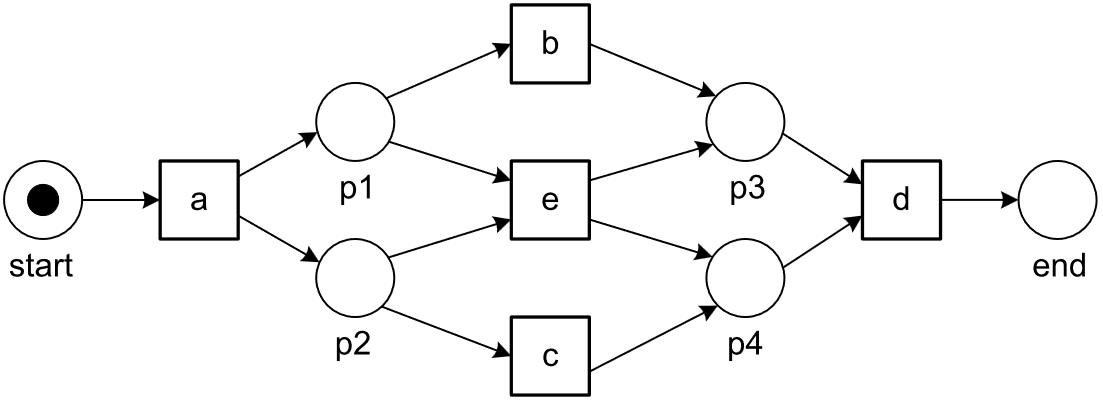
\includegraphics[width=0.5\textwidth]{img/alpha_algorithm_example.png}
                    \end{center}
            \end{enumerate}
        \end{example}

        $\alpha$-algorithm has the following limitations:
        \begin{itemize}
            \item It can learn unnecessarily complex networks.
            \item It cannot learn loops.
            \item The frequency of the traces is not taken into account.
        \end{itemize}


    \item[Model evaluation]
        Different models can capture the same process described in a log.
        This allows for models that are capable of capturing all the possible traces of a log but 
        are unable provide any insight (e.g. flower Petri net).

        \begin{figure}[H]
            \centering
            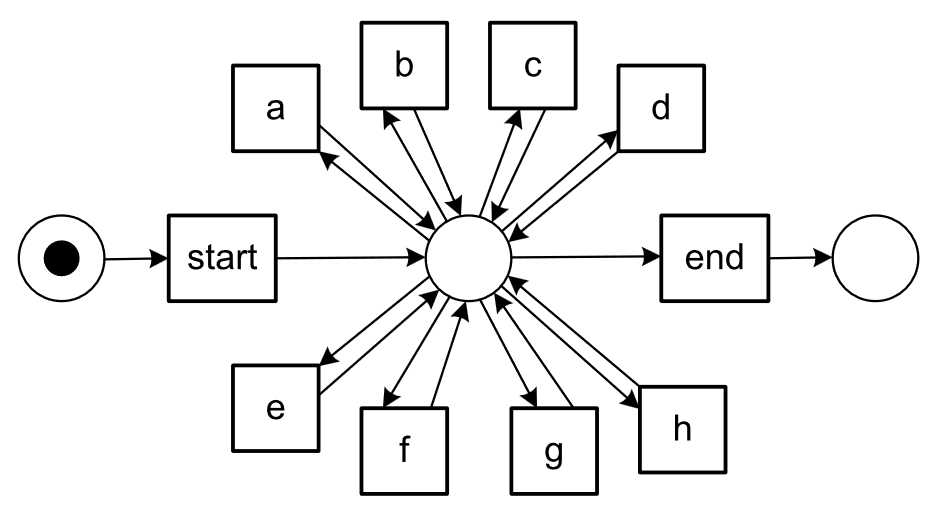
\includegraphics[width=0.4\textwidth]{img/flower_petri.png}
            \caption{Example of flower Petri net}
        \end{figure}

        General judging criteria for a model are:
        \begin{descriptionlist}
            \item[Fitness] \marginnote{Fitness}
                How well the model fits the majority of the traces.
            \item[Simplicity] \marginnote{Simplicity}
                Based on the structure of the model.
            \item[Precision] \marginnote{Precision}
                How the model is able to capture rare cases.
            \item[Generalization] \marginnote{Generalization}
                How the model generalize on the training traces.
        \end{descriptionlist}
\end{description}



\subsection{Conformance checking}

\begin{description}
    \item[Descriptive model discrepancies] \marginnote{Descriptive model}
        The model need to be improved.

    \item[Prescriptive model discrepancies] \marginnote{Prescriptive model}
        The traces need to be checked as the model cannot be changed (e.g. model of the law).
        The deviation of a trace can be desired or undesired.
\end{description}

\begin{remark}
    A trace can be seen as a sequence of symbols. It is possible to syntactically check them using a regular expression.
\end{remark}

\begin{description}
    \item[Token replay] \marginnote{Token replay}
        Given a trace and a Petri net, the trace is replayed on the model by moving tokens around.
        The trace is conform if the end event can be reached, otherwise it is not.

        A modified version of token replay allows to add or remove tokens when the trace is stuck on the Petri net. 
        These external interventions are tracked and used to compute a fitness score (i.e. degree of conformance).

        Limitations:
        \begin{itemize}
            \item Fitness tend to be high for extremely problematic logs.
            \item If there are too many deviations, the model is flooded with tokens and may result in unexpected behaviors.
            \item It is a Petri net specific algorithm.
        \end{itemize}

    \item[Alignment] \marginnote{Alignment}
        Given a trace $l$ and the reference traces $L_\text{ref}$, 
        alignment is based on the edit distance (i.e. minimum number of modifications) between $l$ and the traces in $L_\text{ref}$.

        The fitness score is based on the lowest and highest edit distances.
\end{description}